%\documentclass{article}
%\usepackage{siunitx}
%\usepackage{setspace}
%\usepackage{gensymb}
%\usepackage{xcolor}
%\usepackage{caption}
%\usepackage{subcaption}
%\doublespacing
%\singlespacing
%\usepackage[none]{hyphenat}
%\usepackage{amssymb}
%\usepackage{relsize}
%\usepackage[cmex10]{amsmath}
%\usepackage{mathtools}
%\usepackage{amsmath}
%\usepackage{commath}
%\usepackage{amsthm}
%\interdisplaylinepenalty=2500
%\savesymbol{iint}
%\usepackage{txfonts}
%\restoresymbol{TXF}{iint}
%\usepackage{wasysym}
%\usepackage{amsthm}
%\usepackage{mathrsfs}
%\usepackage{txfonts}
%\let\vec\mathbf{}
%\usepackage{stfloats}
%\usepackage{float}
%\usepackage{cite}
%\usepackage{cases}
%\usepackage{subfig}
%\usepackage{xtab}
%\usepackage{longtable}
%\usepackage{multirow}
%\usepackage{algorithm}
%\usepackage{amssymb}
%\usepackage{algpseudocode}
%\usepackage{enumitem}
%\usepackage{mathtools}
%\usepackage{eenrc}
%\usepackage[framemethod=tikz]{mdframed}
%\usepackage{listings}
%\usepackage{listings}
%\usepackage[latin1]{inputenc}
%\usepackage{color}{   
%\usepackage{lscape}
%\usepackage{textcomp}
%\usepackage{titling}
%\usepackage{hyperref}
%\usepackage{fulbigskip}   
%\usepackage{tikz}
%\usepackage{graphicx}
%\graphicspath{./sdcard/latex/}
%\lstset{
  %frame=single,
 % breaklines=true
%}
%\newcommand{\mydet}[1]{\ensuremath{\begin{vmatrix}#1\end{vmatrix}}}
%\providecommand{\brak}[1]{\ensuremath{\left(#1\right)}}

%\newcommand{\solution}{\noindent \textbf{Solution: }}
%\newcommand{\myvec}[1]{\ensuremath{\begin{pmatrix}#1\end{pmatrix}}}
%\let\vec\mathbf{}

%\title{Geometry Assignment}
%\author{}
%\date{\today}
%\begin{document}
%\maketitle
%\begin{enumerate}
    \item  If a pole $6 m$ high casts a shadow $2\sqrt{3}$  long on the ground,then sun's elevation is:
    \begin{enumerate}[label=(\alph*)]
        \item  $60\degree$
        \item  $45\degree$
        \item  $30\degree$
        \item  $90\degree$
    \end{enumerate}
    \item  In the given \figref{fig:figure2},$\triangle ABC \sim  \triangle QPR$.If $AC= 6 cm$,$BC = 5 cm$, $QR = 3 cm$ and $PR=x$;then the value of $x$is:
        \begin{enumerate}[label=(\alph*)]
            \item  $3.6 cm$
            \item  $2.5 cm$
            \item  $10 cm$
            \item  $3.2 cm$
               \begin{figure}[H]
  \centering
  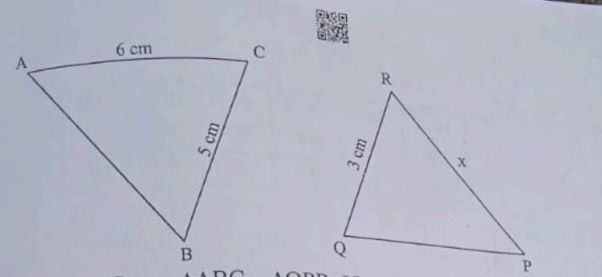
\includegraphics[width=\columnwidth]{figs/triangles.jpeg}
  \caption{}
  \label{fig:figure2}
\end{figure}
        \end{enumerate}
        \pagebreak
    \item  What is the area of a semi-circle of diameter $\lq d \rq$?
    \begin{enumerate}[label=(\alph*)]
        \item  $\frac{1}{16}\pi d^2$
        \item  $\frac{1}{4} \pi d^2$
        \item  $\frac{1}{8}\pi d^2$
        \item  $\frac{1}{2}\pi d^2$
    \end{enumerate}
    \item  In the given \figref{fig:figure1},$PQ \parallel AC$.If $BP = 4 cm$,$AP = 2.4 cm$ and $BQ = 5 cm$,then length of $BC$ is:
    \begin{enumerate}[label=(\alph*)]
        \item $8 cm$
        \item $3 cm$
        \item $0.3 cm$
        \item $\frac{25}{3}cm$
          \begin{figure}[H]
  \centering
  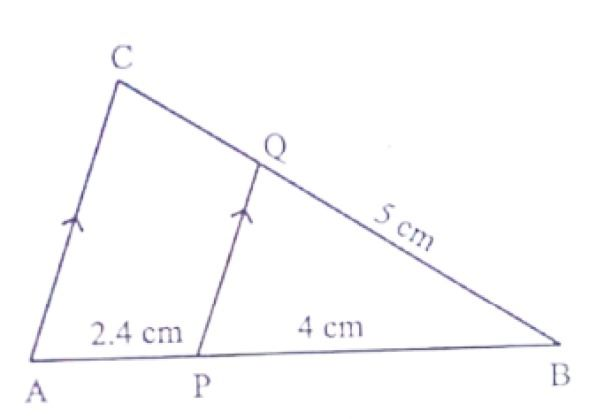
\includegraphics[width=\columnwidth]{figs/right angle triangle.jpeg}
  \caption{}
  \label{fig:figure1}
\end{figure}
    \end{enumerate}
		\pagebreak
       \item  In a $\triangle$  $PQR$,$N$ is a point on $PR$, such that $QN \perp PR$.If $PN \times NR = QN^2$, prove that $\angle PQR = 90 \degree$.
    \item   In the given \figref{fig:figure3}, $\triangle$ $ABC$ and  $\triangle$ $DBC$ are on the same base $BC$ at $O$,prove that
    \begin{align}
         \frac{ar (\triangle  ABC)}{ar (\triangle DBC)} = \frac{AO}{DO}.
    \end{align}
     \begin{figure}[H]
  \centering
  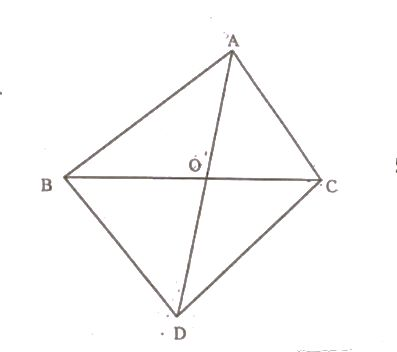
\includegraphics[width=\columnwidth]{figs/square.jpeg}
  \caption{}
  \label{fig:figure3}
\end{figure}
\pagebreak
     \item  A wooden article was made by scooping out a hemisphere from each end of a solid cylinder,as shown \figref{fig:figure4}.If the height of the cylinder is $10 cm$ and its base is of radius $3.5 cm$,find the total surface area of the article.
      \begin{figure}[H]
  \centering
  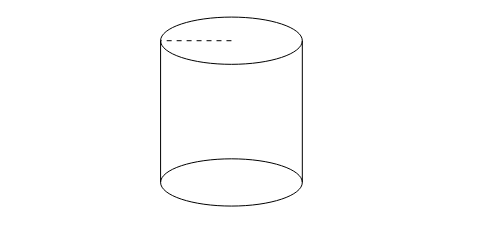
\includegraphics[width=\columnwidth]{figs/cylinder.png}
  \caption{}
  \label{fig:figure4}
\end{figure}
\end{enumerate}
%\end{document}
